\documentclass[conference]{IEEEtran}
\usepackage{graphicx,booktabs,amsmath,cite,url}
% results are \input from files that experiments/run_all.sh copies from results/; until then a visible placeholder prints
\newcommand{\resultinput}[1]{\IfFileExists{#1}{\input{#1}}{\textbf{[pending: #1, run experiments/run\_all.sh]}}}
\newcommand{\resultfig}[1]{\IfFileExists{#1}{\includegraphics[width=\columnwidth]{#1}}{\fbox{\parbox{0.9\columnwidth}{\centering pending: \texttt{#1}}}}}
\begin{document}
\title{VeriRefactor: Verified, Agentic Test-Smell Refactoring with Kill-Set Gating and Detector Consensus}
\author{\IEEEauthorblockN{M Saqib Atif, Gulsher Khan, Hasan Altaf}
\IEEEauthorblockA{Group G2-10, AI4015, FAST-NUCES Islamabad\\
i230769@isb.nu.edu.pk, i230066@isb.nu.edu.pk, i230698@isb.nu.edu.pk\\
IDs: 23I-0769, 23I-0066, 23I-0698}}
\maketitle

\begin{abstract}
Large language models can refactor smelly unit tests, but an accepted refactoring may compile and pass while silently checking less.
UTRefactor, the state of the art, accepts any output that compiles and passes and trusts a single smell detector.
We present VeriRefactor, a multi-agent system in which tools, not the model, decide acceptance.
A Supervisor coordinates Detection, Planner, Refactor and Verifier agents and adapts its next action (retry, switch strategy, narrow targets, revert to the best attempt or escalate) to the Verifier's evidence, with memory of failed approaches within and across tests.
Three components address three gaps: a mutation-testing kill-set gate rejects any refactoring that loses a mutant the original test killed (G1);
smells are targeted and counted as removed only when tsDetect and JNose agree (G2); and adaptive supervision replaces a fixed retry script (G6).
On 150 held-out tests from Commons-cli, Gson and Jsoup, the full system accepts \textbf{[R: results/E3 accepted\_rate]}\% of refactorings with \textbf{[R: accepted\_safe\_rate]}\% accepted and safe,
while switching the gate off lets \textbf{[R: results/E4 H1 s3-G1 pct]}\% of accepted outputs lose mutants. The two detectors disagree sharply on some smells ($\kappa=0.02$ for ExceptionHandling over all 484 tests),
so single-detector reduction rates overstate removal. We release the system, trajectories and scripts that reproduce every table.
\end{abstract}

\section{Introduction}
LLM refactoring of test smells can silently weaken a test: the new code compiles and passes but kills fewer
mutants. UTRefactor~\cite{utrefactor} accepts a refactoring once it compiles and passes. We study three gaps in that setting.
\textbf{RQ1 (G1)}: does a kill-set gate stop accepted refactorings that lose mutants?
\textbf{RQ2 (G2)}: does requiring two detectors (tsDetect, JNose) to agree make smell removal more trustworthy?
\textbf{RQ3 (G6)}: does adaptive supervision (retry, switch strategy, memory) beat a fixed retry script and a single tool-using agent?
Contributions: (i) a verifier that accepts a refactoring only if it compiles, passes, removes the targeted smells and preserves the PIT kill set;
(ii) tsDetect+JNose consensus targets; (iii) an adaptive Supervisor with an LLM planner and cross-test memory;
(iv) a controlled comparison of six systems on 150 held-out tests with 3 seeds.

\section{Related Work}
\emph{Test smells.} Test smells~\cite{garousi2018,tufano2016} are design problems in test code whose harm is debated~\cite{bavota2015}; tsDetect~\cite{peruma2020} and JNose~\cite{virginio2020} detect them, and their agreement is measured with Cohen's $\kappa$~\cite{cohen1960,landis1977}.
UTRefactor~\cite{utrefactor} refactors smells with an LLM and a knowledge base but accepts any output that compiles and passes.
\emph{Mutation testing and oracles.} Mutants are a reasonable proxy for real faults~\cite{just2014}; PIT~\cite{coles2016} computes kill matrices~\cite{jia2011,papadakis2019}, and the oracle problem~\cite{barr2015} motivates preserving the kill-set rather than trusting passing tests. Generated tests~\cite{fraser2011,schafer2024} face the same weakness.
\emph{LLM agents.} Reasoning and acting~\cite{yao2023}, self-feedback~\cite{madaan2023}, verbal memory~\cite{shinn2023}, chain-of-thought~\cite{wei2022}, tool use~\cite{schick2023} and repository agents~\cite{jimenez2024,yang2024} on code models~\cite{chen2021} motivate our Supervisor, but none gates acceptance on mutation evidence.
\emph{Statistics.} We use exact McNemar~\cite{mcnemar1947}, Wilcoxon~\cite{wilcoxon1945} and Wilson intervals~\cite{wilson1927}.

\section{Problem Formulation}
Input: a Java/JUnit project $P$ and a test suite $T=\{t_1,\dots,t_n\}$ (test methods). Smell set $S$ (the tsDetect smells in~\cite{utrefactor}).
Tool set $\mathcal{K}$: for the single-agent baseline \textsf{b2}, $\{\textsf{detect},\textsf{compile\_and\_run},\textsf{pit},\textsf{submit}\}$; \textsf{s3} calls the same tools through its Verifier as one verification step.
For a test $t$, $D(t)\subseteq S$ is its detected smells. A state is $(t, t', D(t'), a)$: original, current candidate,
its smells, and the attempt count $a\le a_{\max}$ (with a per-test token cap). The output is a decision
$d(t)\in\{\text{accept},\text{reject},\text{escalate}\}$ and, if accepted, $t'$.
Constraints: $t'$ compiles and passes; $D(t')\cap D(t)=\emptyset$ for targeted smells; behaviour preservation
$K(t')\supseteq K(t)$ where $K$ is the set of PIT mutants killed. Objective: maximise the rate of accepted-and-safe tests at minimal tokens.

\section{Proposed System}
Figure~\ref{fig:arch} shows the system. A Supervisor drives four agents: Detection (tsDetect, JNose, G2 consensus),
Planner (LLM-written JSON plan with a rule fallback), Refactor (LLM) and Verifier (patch, compile, run, smells, PIT kill-set gate, G1).
The Supervisor accepts, retries, switches strategy, narrows targets, reverts to the best attempt or escalates (G6);
memory holds failed proposals within a test and failed approaches across tests. Every step is logged as a trajectory event.
\begin{table}[t]\centering\caption{Agents, tools and where each gap plugs in.}\label{tab:agents}\footnotesize
\begin{tabular}{@{}lll@{}}\toprule Agent & Tools & Gap\\\midrule
Detection & tsDetect, JNose & G2 (consensus targets)\\
Planner & LLM (JSON plan), KB rule & --\\
Refactor & LLM & --\\
Verifier & javac/JUnit, tsDetect, JNose, PIT & G1 (kill-set gate)\\
Supervisor & memory & G6 (adaptive policy)\\\bottomrule\end{tabular}\end{table}
\textbf{Memory.} Within a test, the Supervisor stores hashes of failed proposals (never re-verified) and the (strategy, gate) pairs that failed; across tests it stores, per project and smell, the planned approaches that failed, and shows them to the Planner.
\begin{figure}[t]\centering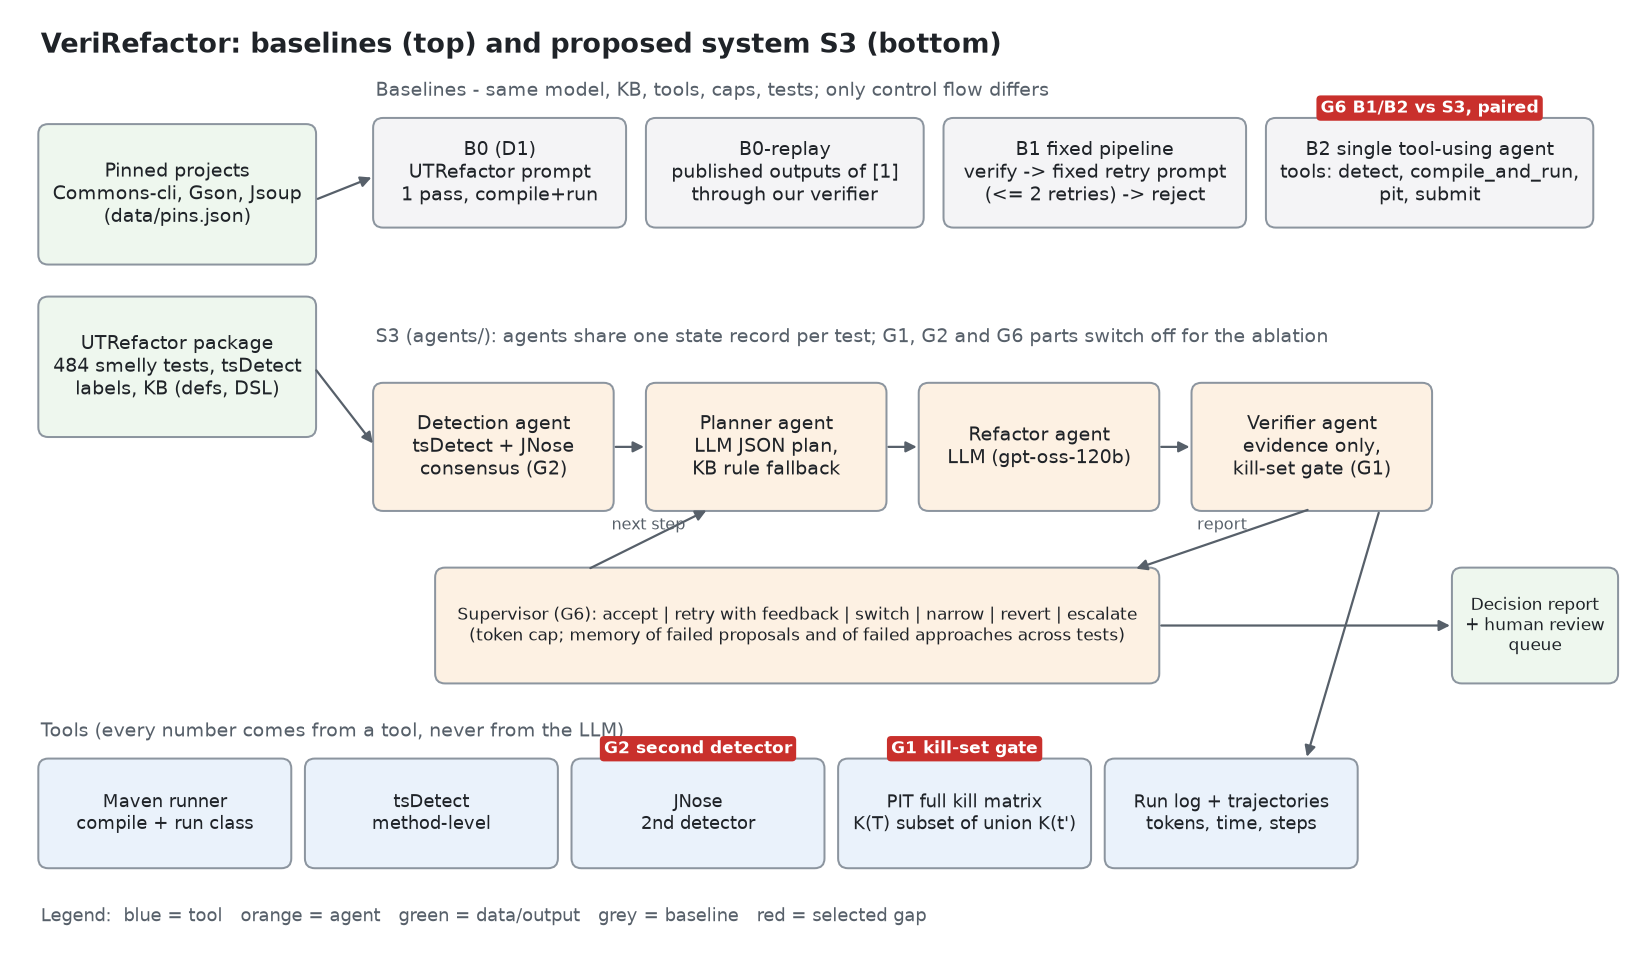
\includegraphics[width=\columnwidth]{architecture.png}
\caption{Architecture and where each gap plugs in.}\label{fig:arch}\end{figure}

\section{Experimental Setup}\label{sec:setup}

\textbf{Benchmark.} We use the test methods of the UTRefactor replication package~\cite{utrefactor}
(Apache Commons-cli, Gson, Jsoup). The package has reports for 492 test methods; 484 match the project commits we pinned
verbatim and form our evaluation set (Commons-cli 77, Gson 238, Jsoup 169; the pinned commits contain 97.9--98.8\% of the published inputs verbatim).
Projects are built at the pinned commit with Maven~3.9.9 (each project with its pinned JDK~17 where its build needs it; JNose and the tool chain run on JDK~21); Gson is evaluated against its own test dependencies at that commit.

\textbf{Splits.} The 484 tests are split once, stratified by project and single/multi-smell, with a fixed seed (commit \texttt{0e1f7da},
\texttt{data/splits/}): \emph{dev} 80 tests (13/39/28 across Commons-cli/Gson/Jsoup), \emph{test} 150 (24/74/52) and \emph{rest} 254 (40/125/89).
Prompts, thresholds, attempt and token caps were tuned on dev only. All reported LLM runs use the test split and the runner's \texttt{--frozen}
guard, which refuses to start from a dirty tree and records the git commit. The rest split is used only for runs without an LLM (E1, E4 detector agreement).

\textbf{Systems.} E1 is UTRefactor's published outputs measured with our verifier (\textsf{b0replay}, no LLM).
E2 compares: \textsf{b0}, UTRefactor's prompt and knowledge base with our model, one pass; \textsf{b1}, the same prompt followed by a fixed retry
script (at most 2 retries with the error text); \textsf{single}, a plain prompt without the knowledge base; \textsf{b2}, a single tool-using agent
with the same tools and token cap as our system; and \textsf{s3}, our multi-agent system. All systems share the model, knowledge base, tools,
per-test token cap and test set. E3 is \textsf{s3} with all three gap components, E5 switches one off at a time
(\textsf{-G1}: kill-set measured, never rejects; \textsf{-G2}: tsDetect only; \textsf{-G6}: fixed retry policy; and memory off).
E2 numbers are labelled \emph{reproduced} when we ran the system and \emph{paper-reported} when they are copied from~\cite{utrefactor}.

\textbf{Model and parameters.} All LLM calls go to Cerebras \texttt{gpt-oss-120b} (free tier, 5 requests/min, 950k tokens/day) at temperature 0.7, at most
8000 output tokens per call and 60\,000 tokens per test. Every configuration on the test split is run with seeds 1, 2 and 3 (see \texttt{experiments/E*.json}), and we report mean $\pm$ sd over them; the replay \textsf{b0replay} calls no LLM and is run once. A sensitivity run (ES) varies the retry cap (0, 1, 2, 4) for \textsf{s3} on the first 20 dev tests; the LLM response cache is keyed by prompt and seed.
Every run records the model ID, temperature, system-prompt hash, seed and git commit in \texttt{config.json} and in the trajectory metadata.

\textbf{Tooling.} tsDetect (v3 jar from the replication package) and JNose (jnose-core 0.9.0, the last release built for Java~21) detect smells at method level;
PIT 1.17.4 computes the full mutation matrix; the fast runner compiles once per Maven module and runs each test class through the JUnit launcher.
The reported runs used an HP Omen~16 laptop with Ubuntu 24.04 under WSL2 (32 logical CPUs and 15~GB of memory visible to Linux), Python~3.12, OpenJDK~17 for the project builds, JDK~21 for JNose and Maven~3.9.9.
The pipeline restores every touched file after each test, and a post-test \texttt{git status} check stops the run if a checkout was left modified.

\textbf{Execution of the reported runs.} All 43 reported runs used the \texttt{--frozen} guard, which refuses to start when a tracked file differs from the commit and records the commit in each run's \texttt{config.json}: the 19 seed-1 runs (and seeds 2--3 of E3 and \textsf{-G1}) were made from commit \texttt{3b992f2}, the 24 seed-2 and seed-3 runs of E2, E5 and ES from \texttt{e9ff1c8}. The two commits share the prompts (same prompt hash), agents, verifier and metrics; the later one adds atomic cache writes, a separate label for runner timeouts, the \texttt{--input} option and the post-hoc JaCoCo check.
To fit the free tier, configurations ran in parallel, each in its own copy of the repository with its own API key, so no two runs ever shared a key or a working directory. A run that hit a key's daily limit was resumed with another key; resumption skips the tests whose results are already saved and redoes only the test in progress.
With up to twelve runs on one machine, PIT used 4 to 8 threads per run. This affects wall-clock times (Table~\ref{tab:e6}); outcomes could change only through PIT's timeout rule, since a slower run can turn a surviving mutant into a timed-out, and therefore killed, one.


\section{Evaluation Methodology}\label{sec:method}

Let $T$ be the evaluated tests, $A\subseteq T$ the accepted ones, and for $t\in T$ let $D(t)$ be its targeted smells (the smells labelled in~\cite{utrefactor}
that the detector in use confirms) and $D'(t)$ the smells still reported in its refactored methods. Rates are percentages; the accepted-losing-mutants rate carries a Wilson 95\% interval.

\textbf{Accepted rate} $=|A|/|T|$. For \textsf{b1}, \textsf{b2} and \textsf{s3} a test is accepted only if the refactoring is statically sane (no dropped or empty test), compiles, passes, and removes the targeted smells;
with G1 on it must also preserve the kill-set. \textsf{single}, \textsf{b0} and \textsf{b0replay} follow~\cite{utrefactor}: accepted if the output compiles and passes (the kill-set is only measured). \textbf{Compile rate} and \textbf{pass rate} are the share of tests whose \emph{last} verification report compiled, respectively passed.

\textbf{Smell reduction} has three definitions. Rule~i (tsDetect, as in~\cite{utrefactor}): $\sum_t|D(t)\setminus D'_{ts}(t)|\,/\,\sum_t|D(t)|$ over all tests; we also report it over accepted tests only.
Rule~ii (strict): a smell counts as removed only if both tsDetect and JNose no longer report it. Rule~iii (manual) is defined in \texttt{labelling\_guide.md}: two labellers judge a 100-test sample independently and Cohen's $\kappa$ measures their agreement. We did not complete this sample before the deadline, so rule~iii is defined but not reported.

\textbf{Behaviour preservation.} For test $t$ let $K(t)$ be the set of PIT mutants killed by $t$, from the full mutation matrix. The original's $K(t)$ is computed on the unmodified class
before the patch is written. A refactoring that yields tests $t'_1..t'_m$ preserves behaviour if $K(t)\subseteq\bigcup_i K(t'_i)$. As a second, weaker check measured after the runs (not a gate), JaCoCo records the main-code lines $L(t)$ the original covers and requires $L(t)\subseteq\bigcup_i L(t'_i)$.
\textbf{Accepted-losing-mutants rate} is the share of accepted tests violating this; \textbf{accepted-and-safe rate} is the share of $T$ that is accepted, preserves $K$, and leaves none of the smells labelled in~\cite{utrefactor} under rule~ii. The last condition uses all labelled smells, not only the targeted ones, so a system that targets fewer smells is not rewarded for leaving the others in place.
Tests with an empty baseline $K(t)$ are counted as \emph{unknown}, not as preserved.

\textbf{Efficiency and reliability.} Tokens per test (total, and split into prompt and completion from the provider's usage field), tokens per accepted test, wall-clock latency per test (includes rate-limit waits), tool calls and retries (reported as totals and per-test means), and
\textbf{recovery rate} $=$ accepted tests among those that needed at least one retry. Cost is \$0 on the free tier; we report tokens instead.

\textbf{Comparison protocol.} Every system runs the same 150 test-split tests. The full system and its \textsf{-G1} variant run with seeds 1, 2 and 3 and are reported as mean $\pm$ sd; the baselines and the other ablations run once (seed 1), because a test-split run with PIT takes several hours. Paired comparisons on the same tests (pooled over seeds where both systems have them) use the exact McNemar test (binary outcomes) and the Wilcoxon
signed-rank test (continuous), with Holm correction across the comparisons in a table and bootstrap confidence intervals for differences.
\textbf{Metric-definition differences from~\cite{utrefactor}:} (i)~our evaluation set has 484 tests (the replication package's reports cover 492 and Table~2 of~\cite{utrefactor} states 593), because the paper does not name its project commits and we pin the commits that contain most of its inputs verbatim; (ii)~we accept an output only if it compiles, passes, removes the targeted smell and (G1) kills every mutant the original killed, whereas rule~i alone credits any output that no longer shows the smell; (iii)~smells are detected per test method; (iv)~Gson is built with its own dependencies. Replaying the published outputs through our verifier (\texttt{b0replay}) matches the paper on Commons-cli (86.4\% against 86\%) but not on Gson (57.9\% against 89\%) or Jsoup (46.0\% against 91\%), Table~\ref{tab:vspaper}; we report these as measured with our build and counting, not as a reproduction of the paper's figures.

% Tables and figures are \input from paper/tables and paper/figures, which experiments/run_all.sh copies from results/.
% Hand-written numbers in the prose are marked \textbf{[R: file]} and must be copied from that file before submission.
\section{Results}\label{sec:results}

Unless stated otherwise, numbers are means $\pm$ sd over the seeds listed in Section~\ref{sec:setup} on the 150-test split, with the same tests for every system.
Table~\ref{tab:systems} compares all systems; every base-paper number is labelled \emph{reproduced} or \emph{paper-reported} (Table~\ref{tab:vspaper}).

\begin{table*}[t]\centering\caption{All systems on the test split (E1--E3). Red.\ i: tsDetect only, as in~\cite{utrefactor}; Red.\ ii: both detectors; Lose mut.: accepted outputs that lose a mutant; Acc.+safe: accepted, kill-set preserved, no targeted smell left.}\label{tab:systems}
\resultinput{tables/E3.tex}\par\smallskip\resultinput{tables/E2.tex}\end{table*}

\begin{table}[t]\centering\caption{Base-paper comparison: rule-i smell reduction (\%) per project, paper-reported~\cite{utrefactor} vs reproduced by us.}\label{tab:vspaper}
\footnotesize\resultinput{tables/E2_vs_paper.tex}\end{table}

\subsection{RQ1 (G1): does the kill-set gate stop weakened tests?}
\textbf{H1:} on tests with a non-empty baseline kill-set, switching the gate off increases the share of accepted refactorings that lose mutants, without a large change in acceptance.
On this subset (\textbf{[R: results/E4/summary.json subsets.H1 n]} tests), accepted outputs losing a mutant are \textbf{[R: H1 s3 pct]}\% with the gate and \textbf{[R: H1 s3-G1 pct]}\% without it,
and acceptance moves from \textbf{[R: s3\_accepted]}\% to \textbf{[R: s3-G1\_accepted]}\%. Paired test (exact McNemar, Holm-corrected): \textbf{[R: paired\_tests ``G1: s3 vs s3-G1'' p\_holm]}.

\subsection{RQ2 (G2): does detector consensus make smell removal more trustworthy?}
\textbf{H2:} the gap between tsDetect-only (rule~i) and strict (rule~ii) smell reduction is largest for the smells where the detectors disagree.
On all 484 originals, JNose confirms 76.2\% of the smells labelled in~\cite{utrefactor} (\texttt{results/E4/g2\_agreement.json}); the detectors agree closely on most smells ($\kappa$ 0.68--1.0)
but not on ExceptionHandling (tsDetect 224, JNose 10, $\kappa=0.02$) or DuplicateAssert ($\kappa=0.42$).
Per smell, rule~i vs rule~ii removal for \textsf{s3} is in \texttt{results/E4/summary.json} (\texttt{H2\_per\_smell\_rule\_i\_vs\_ii}): \textbf{[R: largest gap smell and both percentages]}.

\subsection{RQ3 (G6): does adaptive supervision beat fixed retries and a single agent?}
\textbf{H3:} on multi-smell tests and on hard tests (rejected by the one-pass reproduction \textsf{b0}), \textsf{s3} has a higher accepted-and-safe rate than \textsf{b1} and \textsf{b2} at equal or lower tokens per test.
Accepted-and-safe on multi-smell tests: \textsf{s3} \textbf{[R]}\%, \textsf{b1} \textbf{[R]}\%, \textsf{b2} \textbf{[R]}\%; on hard tests: \textbf{[R]} / \textbf{[R]} / \textbf{[R]}\% (\texttt{H3\_subsets\_accepted\_safe}).
Paired tests \textsf{s3} vs \textsf{b1} and vs \textsf{b2}: \textbf{[R: paired\_tests G6 p\_holm]}.

\subsection{Gap-resolution table}
Table~\ref{tab:gaps} summarises the three gaps; it is generated by \texttt{gap\_table.py} from \texttt{results/} and is identical to the table in the repository README.
\begin{table*}[t]\centering\caption{Gap-resolution table (same as the README).}\label{tab:gaps}\footnotesize\resultinput{tables/gap_table.tex}\end{table*}

\section{Ablation and Comparative Analysis}\label{sec:ablation}
Table~\ref{tab:ablation} switches components off (E5: \textsf{-G1} kill-set measured only, \textsf{-G2} tsDetect targets, \textsf{-G6} fixed retry policy (memory is off with it), \textsf{memory} off, and \textsf{minus\_all} with all three off)
and reports each variant's change from the full system (E3); PIT measures in every variant, so kill-set loss is comparable. Figure~\ref{fig:ablation} plots accepted-and-safe per variant.
\textbf{Sensitivity.} Table~\ref{tab:sensitivity} varies the retry cap (0, 1, 2, 4) for \textsf{s3} on 20 dev tests without PIT (dev only, so it does not touch the test split).
\textbf{Efficiency.} Table~\ref{tab:e6} reports tokens (prompt and completion), LLM and tool calls, wall-clock and PIT time per test, retry and recovery rates for every configuration; cost is \$0 on the Cerebras free tier, and Figure~\ref{fig:cost} relates tokens to accepted-and-safe.

\begin{table*}[t]\centering\caption{Ablation (E5): change from the full system.}\label{tab:ablation}\footnotesize\resultinput{tables/E5_delta.tex}\end{table*}
\begin{table}[t]\centering\caption{Sensitivity to the retry cap (ES, dev split).}\label{tab:sensitivity}\footnotesize\resizebox{\columnwidth}{!}{\resultinput{tables/ES.tex}}\end{table}
\begin{table*}[t]\centering\caption{Efficiency and reliability per configuration (E6), means over seeds.}\label{tab:e6}\footnotesize\resultinput{tables/E6.tex}\end{table*}
\begin{figure}[t]\centering\resultfig{figures/fig_ablation.pdf}\caption{Accepted-and-safe rate of the full system and each ablation.}\label{fig:ablation}\end{figure}
\begin{figure}[t]\centering\resultfig{figures/fig_cost.pdf}\caption{Tokens per test vs accepted-and-safe rate, one point per configuration.}\label{fig:cost}\end{figure}

\section{Failure Analysis}\label{sec:failures}
Each non-accepted test gets exactly one category, assigned from its final verification report by \texttt{failures.py} (the first matching rule wins):
infrastructure error; budget exhausted; malformed reply; assertion dropped or empty test; compile: API not in the project; compile: missing symbol or import; compile: other;
fixture clobbered by extracted setup; semantic change: test now fails; weakened test: kill-set loss; smell not removed or new smell.
Table~\ref{tab:failures} and Figure~\ref{fig:failures} give counts over the three \textsf{s3} seeds (each (test, seed) pair counted once), as a share of failures and of all evaluated pairs.
The largest category is \textbf{[R: results/failures/E3\_counts.json]}.
\begin{table}[t]\centering\caption{Failure modes of the full system (E3, all seeds).}\label{tab:failures}\footnotesize\resizebox{\columnwidth}{!}{\resultinput{tables/failures.tex}}\end{table}
\begin{figure}[t]\centering\resultfig{figures/fig_failures.pdf}\caption{Failure-mode distribution of the full system.}\label{fig:failures}\end{figure}

\textbf{Trajectories.} We walk through two successes and two failures from \texttt{logs/E3\_s3\_s1} (agent $\to$ tool $\to$ result $\to$ decision): the first accepted test that needed a retry, the first clean accept,
and the first rejected test in each of the two largest failure categories (exported with \texttt{failures.py --case}).
\textbf{[R: write from cases/success1.md, success2.md, failure1.md, failure2.md; for each failure give the root cause and the fix]}.

\section{Limitations and Threats to Validity}\label{sec:threats}

\textbf{Internal.} LLM output is non-deterministic even at fixed seeds on a hosted model, and results depend on the prompt and on the retry and token caps, which we tuned on the dev split only;
three seeds bound but do not remove this variance. The free tier limits us to 5 requests per minute and a daily token cap; if a run is resumed on a later day, the hosted model may have changed in between. The reduced seed grid (one seed for most baselines and ablations) leaves those rows without a variance estimate.
PIT results depend on the mutator set and on timeouts: PIT's default behaviour counts a mutant that makes the test time out as killed.

\textbf{External.} Three Java projects (Commons-cli on JUnit~5, Gson and Jsoup on JUnit~4) and 150 held-out tests, with smells restricted to the tsDetect set, do not support claims about other languages, test frameworks or larger suites.
Only one model family (\texttt{gpt-oss-120b}) was used, so the comparison between systems does not show how the gaps behave with a weaker or stronger model.

\textbf{Construct.} The PIT kill-set is a proxy for test strength: the same mutants can be killed by a weaker assertion, and mutants outside the sampled mutators are invisible. tsDetect and JNose disagree sharply on some smells
(ExceptionHandling, IgnoredTest), so ``smell removed'' depends on the detector rule; we report rules~i and~ii, and rule~iii only if the manual sample was completed. Empty baseline kill-sets are reported as unknown rather than safe. JaCoCo coverage, listed as a Phase~1 tool, is not used, so test strength is measured by the kill-set only.
Our evaluation set is 484 tests, not the 593 of~\cite{utrefactor}, because only those match the pinned project commits verbatim.

\section{Conclusion}\label{sec:conclusion}

We built a verified, agentic pipeline that accepts a test-smell refactoring only when it compiles, passes, removes the targeted smells and keeps every mutant the original test killed.
\textbf{G1:} \textbf{[TODO one sentence with the E3 vs E5-G1 number from results/E5]}. \textbf{G2:} \textbf{[TODO detector-consensus finding from results/E4 and E5-G2]}.
\textbf{G6:} \textbf{[TODO s3 vs b1 and b2 from results/E2, E3]}. Architectural lessons: tools, not the model, should decide acceptance; the baseline kill matrix must be computed before the patch is written
(a Phase~1 bug measured the refactored code instead); and failures must be captured per test so one error does not stop a run.
Future work: more projects and models, JaCoCo-style coverage next to the kill-set, parallel workers per project, and a learned planner trained on the cross-test memory.


\bibliographystyle{IEEEtran}
\bibliography{refs}
\end{document}
